\documentclass{article}

\usepackage{microtype}
\usepackage{graphicx}
\usepackage{booktabs}
\usepackage{hyperref}
\usepackage{amsmath}
\usepackage{amssymb}
\usepackage{url}
\usepackage{multirow}
\usepackage{xcolor}
\usepackage{siunitx}
\usepackage[round]{natbib}
\sisetup{detect-weight=true,detect-family=true}

\IfFileExists{icml2025.sty}{\usepackage{icml2025}}{\usepackage{icmlstub}}

\icmltitlerunning{Protocol, Not Architecture}

\begin{document}

\twocolumn[
\icmltitle{Protocol, Not Architecture: What Seven Pipelines on One\\
Predictive-Maintenance Benchmark Actually Measure}

\begin{icmlauthorlist}
\icmlauthor{Anonymous Authors}{anon}
\end{icmlauthorlist}

\icmlaffiliation{anon}{Anonymous Institution}
\icmlkeywords{anomaly detection, time series, benchmarking, evaluation protocol,
predictive maintenance, calibration, distribution shift}

\vskip 0.2in
]

\printAffiliationsAndNotice{\textit{Paper under double-blind review. Do not distribute.}}

\begin{abstract}
We report an audit of a public hydraulic-pump predictive-maintenance benchmark
in which we built seven analysis pipelines (B--G) as separate work-streams over
the same two CSV files, deliberately varying windowing, splitting, threshold
sourcing, scoring unit and post-processing. Reported $F_1$ across these
pipelines spans $0.684$ to $0.988$ --- a range wider than most architecture
comparisons in this literature --- yet no pipeline is meaningfully better at
detection: wherever we measure it under a leakage-controlled protocol, average
precision is $\ge 0.98$ and recall saturates at $1.000$. We isolate the cause.
Holding the network fixed and changing only the protocol moves the official
LSTM-Autoencoder from $F_1 = 0.684$ to $0.988$ in one pipeline and from
$0.743$ to $0.959$ in another. We then show three consequences that any
single-pipeline study would have missed. (i) Detection metrics cannot order
models, but robustness to benign measurement shift separates them by more than
$5\times$ ($+17.0$ vs.\ $+89.7$ percentage points of added false alarms).
(ii) Cross-validated false-alarm rate does not predict deployed false-alarm
rate: on the identical held-out block, five-fold CV reports $0.27\%$ while the
frozen deployment configuration produces $8.23\%$, a $30\times$ gap caused
solely by which block supplies the conformal calibration set. (iii) An anomaly
score that ranks perfectly can still be useless as a probability --- one
pipeline's risk score attains Brier $0.487$ against $0.111$ for a constant
predictor. Finally we show the benchmark's label is confounded with
acquisition session, and that observation length alone bounds detectability
(recall $0.461 \rightarrow 0.821$ as windows grow from 4 to 30 samples). We
argue that packaged reference analyses should report acquisition structure, a
parameter-free baseline, and a measurement-shift stress test, and we explain
why the seven $F_1$ values in this paper must not be ranked against each other.
\end{abstract}

\section{Introduction}
\label{sec:intro}

A public dataset shipped with a reference implementation is a common entry
point into industrial anomaly detection, and the reference score becomes the
number to beat. This paper asks what that number measures.

Our setting is a fine-blanking press hydraulic pump monitored by two vibration
channels and one current channel, distributed with a guidebook implementing an
LSTM-Autoencoder that reports $F_1 = 0.748$ \citep{kamp2022press}. We set out
to beat it. Instead we built seven pipelines, found that essentially all of
them saturate the detection metric, and found that the published number is
reproducible but uninformative.

The seven pipelines (which we label B through G, following their internal
development order) were constructed as separate work-streams with different
design commitments: deep reconstruction models, isolation forests, PCA-based
multivariate statistical process control, shrinkage Mahalanobis monitors, a
one-line range rule, and supervised logistic regression. Crucially they also
differ in \emph{protocol}: window length and whether windows may cross
acquisition gaps; whether splits are random, time-ordered, or blocked by
acquisition burst; whether the decision threshold is fit on normal data alone
or on a validation set containing fault labels; whether scores are evaluated
per row, per window, or per burst; and whether alarms are post-processed.

\textbf{Contributions.}

\textbf{(1) Protocol dominates architecture on this benchmark}
(\S\ref{sec:protocol-effect}). Holding the reference network, optimiser and
epoch budget fixed and changing only preprocessing, windowing, score
aggregation and threshold sourcing moves $F_1$ from $0.684$ to $0.988$ in one
pipeline and from $0.743$ to $0.959$ in another. The $0.743$ figure reproduces
the published $0.748$ to within seed noise, so the gap is not a
reimplementation artefact.

\textbf{(2) Detection saturates, so something else must do the discriminating}
(\S\ref{sec:saturation}). Under a leakage-controlled protocol a parameter-free
range rule reaches $F_1 = 0.973$, higher than every learned model we tested.
Measurement-shift robustness, by contrast, spreads the same models across a
$5\times$ range.

\textbf{(3) Cross-validation does not predict deployment}
(\S\ref{sec:cvgap}). We exhibit a $30\times$ discrepancy on the identical
evaluation block, attributable entirely to the choice of conformal calibration
block --- a direct, quantified failure of exchangeability under blocked
splitting.

\textbf{(4) Perfect ranking is compatible with useless probabilities}
(\S\ref{sec:calib}). A score with $\mathrm{AP} \ge 0.99$ achieves a Brier
score four times worse than predicting the base rate.

\textbf{(5) A negative methodological result} (\S\ref{sec:nocompare}). We
explain why the seven $F_1$ values reported here cannot be assembled into a
ranking, and we decline to do so. We regard publishing the incomparability,
rather than a leaderboard, as the correct output of this study.

We are explicit about what this study is not. The seven pipelines were built by
one group, not by independent teams; this is a protocol-variation study, not a
replication study. The benchmark contains exactly one fault event, recorded
five days after the normal data, so separability is confounded with acquisition
session and no lead-time claim is measurable.

\section{Related Work}
\label{sec:related}

\paragraph{Evaluation pathologies in time-series anomaly detection.}
\citet{kim2022towards} show that the widely used point-adjustment protocol
inflates $F_1$ so severely that random scores appear state-of-the-art.
\citet{wu2023current} argue that several standard benchmarks are trivially
solvable or mislabelled, and \citet{garg2022evaluation} reach similar
conclusions systematically. Our finding is adjacent but distinct: we use no
point adjustment and the labels are not wrong. The benchmark is simply so
separable that the metric stops ordering methods, while protocol choices that
are usually treated as implementation details move the headline number by more
than any architecture choice does.

\paragraph{Shortcut learning and confounded acquisition.}
That models key on nuisance correlates rather than the phenomenon of interest
is documented in vision and medical imaging
\citep{geirhos2020shortcut,zech2018variable}, where site or scanner identity is
easier to predict than pathology; \citet{recht2019imagenet} show how fragile
benchmark conclusions are to distribution details. Here class is perfectly
aligned with acquisition date, which is the starkest possible form.

\paragraph{Classical multivariate process monitoring.} Hotelling's $T^2$ with
squared prediction error is standard for industrial monitoring
\citep{jackson1979control,qin2003statistical} and yields per-variable
contributions for triage. We use it alongside shrinkage covariance estimation
\citep{ledoit2004well} and Isolation Forest \citep{liu2008isolation}.

\paragraph{Distribution-free calibration.} Several of our pipelines set
thresholds by split-conformal $p$-values
\citep{vovk2005algorithmic,angelopoulos2023conformal}. Overlapping windows
violate exchangeability, so we block by acquisition burst in the spirit of
purged cross-validation \citep{lopezdeprado2018advances}; \S\ref{sec:cvgap}
quantifies what happens when that is not enough.

\section{Problem Formulation}
\label{sec:prelim}

The claim of this paper is that the reported number is a function of the
protocol, not only of the model. To state that precisely we have to give the
protocol its own notation, which the usual time-series anomaly detection (TAD)
formulation leaves implicit.

\subsection{Signals, sessions and labels}

Let $X=(x_1,\dots,x_T)$, $x_t\in\mathbb{R}^{N}$ with $N=3$, be the record
observed at timestamps $\tau_1<\dots<\tau_T$, and write
$\Delta_t=\tau_{t+1}-\tau_t$. A label $y_t\in\{0,1\}$ marks fault.

Two facts about this benchmark enter the notation because every pipeline
inherits them. The label is constant within each file, so it is a property of
the record rather than of the sample; and writing $c(t)\in\{1,2\}$ for the
acquisition session, $y_t=\mathbb{1}[c(t)=2]$ holds exactly. Session and label
are perfectly confounded (\S\ref{sec:limits}).

\subsection{Acquisition bursts}

The standard formulation assumes $\Delta_t$ constant. Fix a gap threshold $g$
and define the acquisition bursts as the maximal runs
\begin{equation}
\mathcal{B}=\{B_1,\dots,B_K\},\quad
B_k=\{t: a_k\le t\le b_k\},\ \Delta_t\le g\ \forall t\in[a_k,b_k),
\label{eq:burst}
\end{equation}
with $g=\SI{0.5}{\second}$. Section~\ref{sec:data} shows $K=599$ for the normal
record with bursts of at most 50 samples.

\subsection{A protocol is a tuple}
\label{sub:tuple}

Each pipeline in this study is an instance of
\begin{equation}
\Pi \;=\; \bigl(\ell,\ \gamma,\ \mathcal{U},\ \sigma,\ \Theta,\ \pi\bigr),
\label{eq:protocol}
\end{equation}
whose components are exactly the columns of Table~\ref{tab:protocols}:

\begin{description}\itemsep1pt
\item[$\ell$] window length in samples (4 to 30 across pipelines; ``native''
  for burst-level scoring).
\item[$\gamma\in\{0,1\}$] \emph{gap-safety}. With $\gamma=1$ a window is
  admitted only if $[t,t+\ell-1]\subseteq B_k$ for some $k$; with $\gamma=0$
  windows may straddle gaps. Define the survival rate
  $\rho(\ell)=|\mathcal{W}^{\gamma=1}_\ell|/|\mathcal{W}^{\gamma=0}_\ell|$.
\item[$\mathcal{U}$] \emph{scoring unit}: window, row, or burst. This fixes
  what one observation is, and hence what $\mathrm{TP}$ counts.
\item[$\sigma$] \emph{split rule}: which data fit the model, which calibrate
  the threshold, which are held out, and whether blocks respect burst
  boundaries.
\item[$\Theta$] \emph{threshold source}: normal data only (conformal or
  quantile), normal $+$ fault, or supervised cross-validation.
\item[$\pi$] \emph{post-processing}, in particular the persistence operator
\begin{equation}
\Pi^{\mathrm{pers}}_{N_{\mathrm w},M}(\hat y)_t=\mathbb{1}\!\left[\textstyle\sum_{j=t-N_{\mathrm w}+1}^{t}\hat y_j\ \ge M\right],
\label{eq:mofn}
\end{equation}
evaluated inside one burst. Pipeline~D uses $N_{\mathrm w}=M=3$; pipeline~F
uses the loose form $(N_{\mathrm w},M)=(3,2)$.
\end{description}

A detector proper is a score $A:\mathbb{R}^{d}\!\to\mathbb{R}$ fitted on normal
data, thresholded to give $\hat y$. \textbf{The thesis of this paper is that
varying $\Pi$ with $A$ held fixed moves the reported $F_1$ further than varying
$A$ with $\Pi$ held fixed} (\S\ref{sec:protocol-effect}), so the seven
numbers in the last column of Table~\ref{tab:protocols} are not comparable:
they are measurements of seven different $\Pi$.

\subsection{Evaluation levels and effective sample size}
\label{sub:levels}

Because $\mathcal{U}$ differs across pipelines, we name the three granularities
explicitly. $\mathcal{L}_1$ counts windows or rows; overlapping windows share
$\ell-1$ of $\ell$ samples and are not independent. $\mathcal{L}_2$ counts
bursts, the smallest plausibly exchangeable unit. $\mathcal{L}_3$ counts
maximal runs of alarming units as alarm events, which is where false alarms per
hour are defined. A pipeline reporting $\mathcal{L}_1$ $F_1$ and one reporting
$\mathcal{L}_2$ $F_1$ are not measuring the same quantity even on identical
predictions.

The effective number of positive observations is not $|\{t:y_t=1\}|$ but the
number of independent fault events, which is \textbf{one}. Interval estimates
that resample units rather than bursts are therefore not valid here.

\subsection{Point adjustment}
\label{sub:pa}

Let $\mathcal{S}=\{S_1,\dots,S_M\}$ be the fault segments. The point-adjustment
protocol \citep{kim2022towards} sets $\hat y^{\mathrm{PA}}_t=1$ for all $t\in
S_m$ whenever $\hat y_{t'}=1$ for some $t'\in S_m$. It can only raise
$\mathrm{TP}$ and lower $\mathrm{FN}$, so $F_1^{\mathrm{PA}}\ge F_1$ always.
\textbf{No pipeline in this study uses it}, and \S\ref{sec:protoval} measures
what it would have done.

\section{The Benchmark}
\label{sec:data}

The package contains a normal record of $20{,}000$ rows (2022-07-12) and a
fault record of $600$ rows (2022-07-17), each with upper and lower pump
vibration (\texttt{AI0}, \texttt{AI1}), motor current (\texttt{AI2}), and an
equipment-state flag that is constant within each file. Sampling is documented
as \SI{10}{\hertz}.

\paragraph{Acquisition is burst-sampled.} The normal file spans
\SI{4615.8}{\second} of wall-clock time while containing only
\SI{2000}{\second} of samples at \SI{10}{\hertz}; 598 inter-sample gaps exceed
\SI{0.5}{\second}. Segmenting there yields 599 bursts, median 37 and maximum
50 samples --- at most \SI{4.9}{\second} of contiguous signal. The fault file
has 21 bursts, maximum 50 samples. \textbf{No burst reaches the 120 samples
that the reference pipeline's 20-sample window plus 100-step label offset
spans} (Figure~\ref{fig:burst}), so that pipeline's windows necessarily cross
gaps and its stated \SI{10}{\second} horizon is unrealizable. Restricting
windows to lie inside one burst removes $25.6\%$ of windows at length 10 and
$50.1\%$ at length 20.

\begin{figure}[t]
\centering
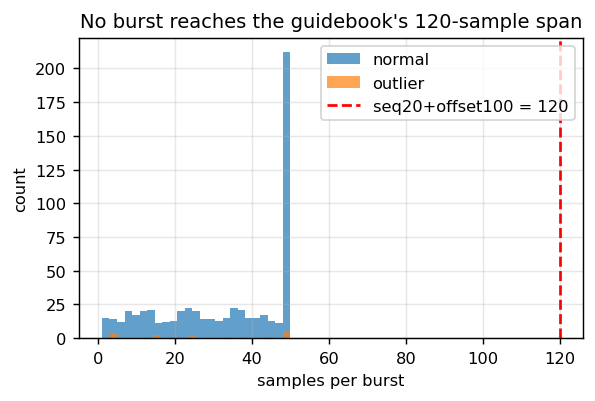
\includegraphics[width=\columnwidth]{figures/fig2_burst_length.png}
\caption{Burst length distribution. The reference analysis span (120 samples,
dashed) exceeds every burst in both files.}
\label{fig:burst}
\end{figure}

\paragraph{One fault event, confounded with date.} The fault file is a single
uninterrupted recording of an already-faulted machine. Its 428 windows (at
length 10) are overlapping fragments of \emph{one} event, not 428 independent
positives, and no pre-failure segment exists. Normal and fault were recorded
five days apart, so load, tooling, product and sensor state are free to differ.
Every separability result below must be read against this.

\paragraph{A preprocessing step that removes the deep model's advantage.} The
reference pipeline applies $|\cdot|$ to all three channels. Window RMS is
\emph{exactly} invariant to this ($|x|^2 = x^2$), as are mean absolute value
and peak: measured over $14{,}871$ normal windows the maximum change in each is
$0.0$. What the transform destroys is sign and phase --- window standard
deviation changes by up to $1.19\times10^{2}$, signed mean by
$2.78\times10^{2}$, peak-to-peak by $3.04\times10^{2}$ and kurtosis by $4.88$.
The signed mean matters: the fault record's current channel carries a large DC
offset that $|\cdot|$ confounds with an amplitude increase. The reference thus
discards the only information a sequence model could exploit that a
moment-based monitor cannot, before training the sequence model.

\section{Seven Pipelines}
\label{sec:pipelines}

Table~\ref{tab:protocols} summarises how the pipelines differ. The differences
are not incidental: each row changes what the reported number means.

\begin{table*}[t]
\caption{Protocol matrix. ``Gap-safe'' means windows may not cross an
acquisition gap. ``Threshold data'' is what the decision threshold was fit on.
The last column is each pipeline's own headline $F_1$; \S\ref{sec:nocompare}
explains why these must not be compared.}
\label{tab:protocols}
\vskip 0.1in
\centering
\small
\begin{tabular}{llllllr}
\toprule
Pipeline & Model family & Unit & Window & Gap-safe & Threshold data & Own $F_1$ \\
\midrule
B  & LSTM-AE ablations        & window & 20     & varies by arm & varies by arm  & 0.684--0.988 \\
C  & Isolation Forest         & window & 10     & yes & normal + persistence   & 0.949 \\
D  & PCA-MSPC (+ 4 baselines) & window & 10     & yes & normal only (conformal) & 0.962 \\
E  & PCA $Q$-statistic        & row    & 20     & \textbf{no}  & normal, locked split & 0.958 \\
F  & PCA + 2-of-3 alarm       & row    & 20     & \textbf{no}  & normal, locked split & 0.918 \\
G  & Logistic regression      & burst  & native & n/a & supervised CV          & 0.942 \\
\bottomrule
\end{tabular}
\end{table*}

Pipeline~D additionally reproduces the reference LSTM-Autoencoder exactly
($64\!\to\!32\!\to$ repeat $\to\!32\!\to\!64$) in two configurations, G0
following the guidebook and G1 inside D's own protocol, which gives us a
controlled architecture-held-fixed comparison. Pipeline~B independently ablates
the same network one factor at a time.

\section{Protocol Dominates Architecture}
\label{sec:protocol-effect}

Table~\ref{tab:protocol-effect} reports both controlled experiments. In
pipeline~B, changing only the score aggregation (last-timestep to whole-window
MSE) raises $F_1$ from $0.684$ to $0.826$; fitting the threshold on normal data
alone instead drives false positives to zero but recall to $0.537$; combining
all structural corrections yields $F_1 = 0.988 \pm 0.001$. In pipeline~D, the
guidebook configuration reproduces the published result
($0.743 \pm 0.029$ vs.\ published $0.748$; precision, recall and FPR all within
seed noise), and the same network inside D's protocol reaches $0.959$.

\begin{table}[t]
\caption{Same architecture, different protocol. B arms are $3$ seeds; D rows
are $3$ seeds (G0) and $5$ folds (G1). Published row from
\citet{kamp2022press}.}
\label{tab:protocol-effect}
\vskip 0.08in
\centering
\small
\setlength{\tabcolsep}{4pt}
\begin{tabular}{llrrr}
\toprule
 & Change from reference & Recall & FPR & $F_1$ \\
\midrule
\multicolumn{5}{l}{\textit{Published}} \\
\quad --- & --- & 0.856 & 0.0195 & 0.748 \\
\midrule
\multicolumn{5}{l}{\textit{Pipeline B (one factor at a time)}} \\
\quad G0 & none (reference)        & 0.813 & 0.0254 & 0.684 \\
\quad A3 & whole-window MSE        & 0.872 & 0.0108 & 0.826 \\
\quad A4 & normal-only threshold   & 0.537 & 0.0000 & 0.697 \\
\quad P20 & all corrections        & 0.993 & 0.0019 & \textbf{0.988} \\
\midrule
\multicolumn{5}{l}{\textit{Pipeline D (exact reproduction)}} \\
\quad G0 & none (reference)        & 0.843 & 0.0193 & 0.743 \\
\quad G1 & D's protocol            & 1.000 & 0.0127 & \textbf{0.959} \\
\bottomrule
\end{tabular}
\end{table}

Two independent routes therefore give the same answer: on this benchmark the
evaluation protocol is the first-order variable and the architecture is not.
We also note that under G0 early stopping never fired --- all three seeds
consumed the full 800-epoch budget despite a patience of 40 on training loss
--- whereas G1 stopped between 499 and 679 epochs.

\section{Detection Saturates}
\label{sec:saturation}

Table~\ref{tab:saturation} gives pipeline~D's five-fold comparison, the only
place in this study where several model families are evaluated under one
protocol. A parameter-free range rule (BL-0) that merely checks whether
features leave their training min--max attains $F_1 = 0.973$, higher than every
learned model including the reference network. Average precision is $\ge 0.98$
for all five and $1.000$ for three.

\begin{table}[t]
\caption{One protocol, five model families (pipeline~D, five-fold block CV,
window unit, prevalence $\approx 12\%$). Detection saturates; the models are
ordered only by false alarms and by shift robustness.}
\label{tab:saturation}
\vskip 0.08in
\centering
\small
\setlength{\tabcolsep}{3.5pt}
\begin{tabular}{lrrrrr}
\toprule
 & Recall & AP & $F_1$ & FP rate & Shift \\
 &  &  &  & (worst) & (worst) \\
\midrule
BL-0 range rule   & 1.000 & 1.000 & \textbf{0.973} & 0.0201 & $+61.3$ \\
M1 Mahalanobis    & 1.000 & 1.000 & 0.965 & 0.0219 & $+89.7$ \\
M2 Isolation For. & 0.932 & 0.983 & 0.929 & 0.0222 & $+22.3$ \\
M3 PCA-MSPC       & 1.000 & 0.999 & 0.962 & 0.0227 & $\mathbf{+17.0}$ \\
BL-1 LSTM-AE (G1) & 1.000 & 1.000 & 0.959 & 0.0268 & n/e \\
\bottomrule
\end{tabular}
\end{table}

\paragraph{Where the separability comes from.} Ablating feature groups, shape
features alone give $\mathrm{AP} = 0.9986$ and amplitude features alone
$0.9935$, while sensor-relation and current-level features alone give $0.6923$
and $0.5052$. Removing any single group leaves AP above $0.98$. Redundancy
across groups of this kind is the signature of a global difference between two
recordings, not of a localized fault mechanism.

\paragraph{What does discriminate.} We perturbed \emph{normal} held-out data
with sensor gain, DC offset, polarity inversion and sampling jitter --- changes
a maintenance monitor must not report as equipment faults --- and measured the
increase in false-alarm rate (last column of Table~\ref{tab:saturation},
Figure~\ref{fig:robust}). A DC offset of half a training standard deviation
drives the Mahalanobis monitor from $\approx 2\%$ to $89.8\%$ of normal windows
flagged; the range rule collapses under gain change; PCA-MSPC is most stable at
$+17.0$ points. Recall on fault data is essentially unaffected for all three
($\le 2.4$ points), precisely because recall is already saturated --- which is
why the perturbation test is informative only on the normal side.

\begin{figure}[t]
\centering
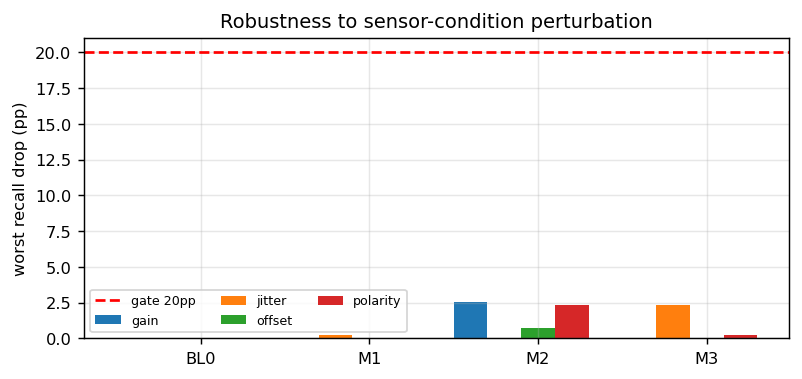
\includegraphics[width=\columnwidth]{figures/fig5_robustness.png}
\caption{Robustness to benign measurement perturbation. Models that are
indistinguishable in Table~\ref{tab:saturation} differ by more than $5\times$.}
\label{fig:robust}
\end{figure}

\paragraph{A caveat we must state.} The shift gate was not evaluated for the
LSTM-Autoencoder (marked n/e): the perturbation study requires retraining for
every fold$\times$perturbation combination, and a single five-fold run of that
network costs \SI{3.6}{\hour} on CPU, exceeding our budget by more than an
order of magnitude. Its exclusion from our preferred configuration rests on the
false-alarm column alone.

\section{Cross-Validation Does Not Predict Deployment}
\label{sec:cvgap}

This is the result we did not anticipate and would have missed with a single
pipeline.

Pipeline~D freezes a deployment configuration: fit on normal blocks 0--2,
conformal calibration on block 3, leaving block 4 never seen. On block 4 the
frozen system raises a first-stage alarm on $241/2929 = \mathbf{8.23\%}$ of
normal windows. The five-fold cross-validation that selected this model
reports, \emph{on the identical block 4}, a false-positive rate of
$8/2929 = \mathbf{0.27\%}$. The gap is $30\times$.

Nothing about the model differs. The CV fold that holds out block 4 calibrates
on block 0; the frozen configuration calibrates on block 3. Block 3 happens to
be a quiet stretch, so the quantile it supplies is too tight for block 4, which
contains a change in operating regime. Of the 241 non-green windows, 217 fall
in original rows $16{,}000$--$19{,}000$, and $54$ of block 4's $106$ bursts
raise at least one alarm.

This is a direct, quantified failure of the exchangeability assumption that
split-conformal inference requires, arising from blocked rather than random
splitting --- exactly the splitting that burst structure forces on us. The
practical consequence is that \textbf{a cross-validated false-alarm rate is not
a property of the system}; it is a property of the (fold, calibration block)
pair. We know of no way to repair this with the data available: with five
blocks and one fault event there is no held-out budget left to estimate the
deployment configuration's false-alarm rate honestly.

\paragraph{Consequence for headline numbers.} Recomputing on the frozen
system's own prediction file (held-out normal block plus fault record,
prevalence $12.75\%$) gives first-stage $F_1 = 0.780$ at
$\mathrm{FPR} = 0.082$. A two-stage rule that additionally requires a
vibration-only monitor to agree for three consecutive windows gives
$F_1 = 0.931$, recall $0.876$, and $\mathrm{FPR} = 0.0010$ --- three false
alarms in $2929$ windows. The CV average of $0.962$ describes neither.

\section{Perfect Ranking, Useless Probabilities}
\label{sec:calib}

Pipeline~D exposes $\mathrm{risk} = 1 - p_{\text{normal}}$, where
$p_{\text{normal}}$ is a split-conformal $p$-value. On the frozen evaluation
set this score has $\mathrm{AP} \ge 0.99$ --- it ranks almost perfectly --- yet
its Brier score is $\mathbf{0.487}$ against $\mathbf{0.111}$ for a constant
predictor at the base rate, and its log-loss is $1.695$. Of normal held-out
windows, $73.1\%$ receive $\mathrm{risk} > 0.5$. A conformal $p$-value is
uniform under the null \emph{by construction}, so $1-p$ concentrates near $1$
for normal data; it is a rank statistic and reporting it as a probability is a
category error, however good the ranking.

Realized conformal coverage shows a second, model-dependent failure
(Table~\ref{tab:coverage}): three monitors track the nominal level within
$0.017$ at $\alpha = 0.10$, but the range rule saturates at $0.013$ regardless
of $\alpha$, because every window inside the training range receives an
identical score of zero and the $p$-value has no resolution below the tie mass.
A model whose threshold cannot be read as a probability is unusable for alarm
budgeting --- and this is invisible in Table~\ref{tab:saturation}, where that
same model has the best $F_1$.

\begin{table}[t]
\caption{Realized conformal coverage $\Pr(p \le \alpha)$ on normal hold-out,
averaged over folds.}
\label{tab:coverage}
\vskip 0.08in
\centering
\small
\begin{tabular}{lrrr}
\toprule
$\alpha$ & 0.01 & 0.05 & 0.10 \\
\midrule
BL-0 range rule   & 0.008 & 0.012 & 0.013 \\
M1 Mahalanobis    & 0.010 & 0.047 & 0.098 \\
M2 Isolation For. & 0.011 & 0.065 & 0.116 \\
M3 PCA-MSPC       & 0.012 & 0.052 & 0.113 \\
\bottomrule
\end{tabular}
\end{table}

By contrast pipeline~E, which fits a sigmoid to its PCA $Q$-statistic, reports
Brier $0.00198$ and log-loss $0.0161$ on its own locked split. Calibration is
therefore achievable on this data --- it simply does not come free with a good
ranking, and no pipeline that reported only $F_1$ would have noticed the
difference.

\section{Observation Length Bounds Detectability}
\label{sec:length}

Pipeline~G (supervised logistic regression on five window statistics,
$50$-fold CV, burst unit) attains recall $0.900$ and $F_1 = 0.942$ with zero
false positives, and its $20$ false negatives fall entirely on two bursts of
length $10$ and $15$. Cropping bursts to a fixed sample count with the model
frozen gives the curve in Table~\ref{tab:length}: recall rises monotonically
from $0.461$ at four samples to $0.821$ at thirty.

\begin{table}[t]
\caption{Recall vs.\ available observation length (pipeline~G, frozen model,
out-of-fold crops). Detectability is bounded by how much contiguous signal a
burst provides.}
\label{tab:length}
\vskip 0.08in
\centering
\small
\begin{tabular}{lrrrrrr}
\toprule
Samples   & 4 & 8 & 10 & 15 & 20 & 30 \\
\midrule
Recall    & 0.461 & 0.467 & 0.529 & 0.682 & 0.749 & 0.821 \\
$F_1$     & 0.631 & 0.637 & 0.692 & 0.811 & 0.856 & 0.902 \\
\bottomrule
\end{tabular}
\end{table}

This reframes those false negatives. They are not model errors to be tuned
away but a statement about information: below roughly $\SI{1.5}{\second}$ of
contiguous signal this feature set cannot decide. The operational implication
is that a short burst should yield \emph{abstention} rather than a negative
classification --- a distinction no aggregate $F_1$ expresses.

\section{What the Protocol Choices Are Worth}
\label{sec:protoval}

Sections~\ref{sec:protocol-effect}--\ref{sec:length} show that $\Pi$ moves
the headline number. We now price two specific components of $\Pi$ that are
easy to omit: the reference baseline, and the post-processing operator $\pi$.
Both are measured on pipeline~D, which is the only one whose per-window scores,
conformal $p$-values and burst indices are all retained; the mechanisms,
however, are properties of the protocol and apply to any pipeline sharing the
relevant component.

\subsection{A trivial baseline, and point adjustment}

\begin{table}[t]
\caption{Oracle $F_1$ on D's hold-out ($2{,}929$ normal windows, $428$ fault
windows in $17$ segments). Random scores averaged over 20 seeds.}
\label{tab:protoval}
\vskip 0.1in
\centering\small
\setlength{\tabcolsep}{4pt}
\begin{tabular}{@{}llr@{}}
\toprule
Score & Prot. & $F_1$ \\
\midrule
D stage-1, oracle $\delta$ & --- & 0.994 \\
Uniform random, oracle $\delta$ & --- & 0.228\,$\pm$\,0.002 \\
D stage-1, conformal $\alpha{=}0.01$ & --- & 0.780 \\
\midrule
D stage-1, oracle $\delta$ & PA & 1.000 \\
Uniform random, oracle $\delta$ & PA & \textbf{0.779\,$\pm$\,0.041} \\
\bottomrule
\end{tabular}
\end{table}

Against a uniform random score the detector is clearly separated,
$F_1=0.994$ versus $0.228$ (Table~\ref{tab:protoval}). Under point adjustment
(\S\ref{sub:pa}) a \emph{random} score reaches $0.779\pm0.041$, which is
indistinguishable from the operational $F_1=0.780$ of the deployed system. The
inflation grows as segments shorten --- restricting to the shortest quarter of
fault bursts (median 6 windows) raises a random score from $0.030$ to $0.173$,
a factor of $5.8$ --- because PA converts one chance hit into credit for an
entire segment regardless of its length.

This bears directly on \S\ref{sec:nocompare}. The seven $F_1$ values in
Table~\ref{tab:protocols} already span $0.684$--$0.988$ from protocol variation
alone; had any pipeline additionally adopted PA, its number would have moved
into the same range for reasons having nothing to do with its model. A
packaged benchmark that does not state its adjustment convention cannot be
compared against at all.

\subsection{Loose persistence does not help}
\label{sec:mofn}

Pipelines D and F differ in $\pi$: D requires three consecutive alarms,
F requires two of three. The loose form is the usual recommendation, on the
reasoning that it tolerates quiet stretches inside a fault. We measure the
whole family on D.

\begin{table}[t]
\caption{Persistence rules on D's hold-out. Candidates satisfy both stages at
$\alpha=0.01$; index windows never cross a burst boundary.}
\label{tab:mofn}
\vskip 0.1in
\centering\small
\setlength{\tabcolsep}{4pt}
\begin{tabular}{@{}lccccc@{}}
\toprule
Rule & Bursts & $R_{\mathcal{L}_1}$ & FP win. & FP ev. & Delay \\
\midrule
consec.\ 1 & \textbf{16/17} & 0.963 & 35 & 23 & \SI{0.0}{\second} \\
consec.\ 2 & 15/17 & 0.916 & 12 & 9 & \SI{0.1}{\second} \\
\textbf{2 of 3} \small(F) & 15/17 & 0.893 & \textbf{23} & 8 & \SI{0.2}{\second} \\
\textbf{consec.\ 3} \small(D) & 15/17 & 0.876 & \textbf{3} & 2 & \SI{0.2}{\second} \\
3 of 4 & 15/17 & 0.853 & 8 & 3 & \SI{0.3}{\second} \\
3 of 5 & 15/17 & 0.829 & 15 & 5 & \SI{0.4}{\second} \\
4 of 5 & 15/17 & 0.811 & 4 & 1 & \SI{0.4}{\second} \\
consec.\ 5 & 14/17 & 0.799 & \textbf{0} & 0 & \SI{0.4}{\second} \\
\bottomrule
\end{tabular}
\end{table}

Table~\ref{tab:mofn} reverses the recommendation. Loosening from
\emph{consecutive 3} to \emph{2 of 3} multiplies false-alarm windows by
$7.7\times$ ($3\to23$) while detecting the same 15 of 17 bursts; the same holds
at $N_{\mathrm w}=5$ ($0\to15$). The normal hold-out contains 35 isolated
candidate windows scattered across the record, so widening the index window
mostly brings \emph{distinct} candidates into one frame rather than bridging a
genuine fault. We state the limitation plainly: this is measured under D's
$(\ell=10,\gamma=1,\mathcal{U}=\text{window})$, whereas F scores rows with
$\gamma=0$, so it is evidence that F's choice deserves re-examination rather
than a demonstration that F is wrong.

A second reading changes the framing. With stride \SI{0.1}{\second} the median
detection delay moves only from \SI{0.0}{\second} to \SI{0.4}{\second} across
the entire family, negligible against the \SI{8}{\second} burst period.
\textbf{The operative trade-off is not delay against false alarms but misses
against false alarms} --- and on that axis the parameter that matters is
$N_{\mathrm w}$, not $M/N_{\mathrm w}$.

\section{Why These Numbers Must Not Be Ranked}
\label{sec:nocompare}

It is tempting to read the last column of Table~\ref{tab:protocols} as a
leaderboard. It is not one, for reasons we think generalise.

\textbf{The unit differs.} D scores windows (prevalence $\approx 12\%$), E and
F score rows (prevalence $8.2\%$), G scores bursts (prevalence $3.4\%$). $F_1$
depends on prevalence, so these are different quantities with the same name.

\textbf{The positive count differs by construction.} D's 428 fault windows, E
and F's 357 positive rows, and G's fault bursts are different partitions of
\emph{one} event. None are independent samples, so no confidence interval
computed over them describes uncertainty about faults.

\textbf{Window validity differs.} E's and F's main models use 20-row
index-contiguous windows that cross acquisition gaps; a 20-row window can span
more than \SI{20}{\second} of wall-clock time. Their scores are computed on
inputs that pipeline~D's analysis (\S\ref{sec:data}) identifies as artefacts.
We report their numbers because they are what those pipelines produced, not
because we endorse the inputs.

\textbf{Selection is entangled across pipelines.} E was developed after F's
final evaluation and uses the same test rows, so E's locked-split guarantee
does not survive the cross-pipeline view.

\textbf{Post-processing changes the operating point, not the model.} F's
headline zero false positives comes from a 2-of-3 alarm rule that also reduced
true positives from $315$ to $303$, moving $F_1$ from $0.936$ to $0.918$.
Reporting the zero without the cost would misstate the trade-off.

We therefore report the spread and refuse the ranking. In our view this is the
honest output: a benchmark on which seven protocols yield $F_1 \in
[0.684, 0.988]$ with no detection difference is not measuring model quality,
and presenting a winner would manufacture a finding the data cannot support.

\paragraph{What can be compared.} The refusal is specific to \emph{across}
pipelines. Comparison is well defined \emph{within} a protocol, and exactly one
of our pipelines supplies one: pipeline~D evaluates five model families ---
including a parameter-free baseline and the reference LSTM-Autoencoder --- on
identical windows, identical folds, and a calibration set drawn only from
normal data (Table~\ref{tab:saturation}). That table is the only comparison in
this study whose differences are attributable to the models rather than to
their evaluation. Its lesson is not that one family wins on $F_1$: the
parameter-free rule has the highest $F_1$ and is nonetheless the worst choice,
failing both the shift test (\S\ref{sec:saturation}) and the calibration test
(\S\ref{sec:calib}). The lesson is that once a single protocol is enforced,
the ordering must come from false alarms under shift and from calibration,
because detection no longer discriminates. We regard ``fix one protocol, then
rank on robustness and calibration rather than on $F_1$'' as the transferable
recommendation of this paper.

\section{Threats to Validity}
\label{sec:limits}

The seven pipelines were built by one group over one dataset; this is a
protocol-variation study, not an independent replication, and shared
assumptions may have propagated. Several pipelines observed the fault record
during exploratory work before their protocols were fixed, so none should be
read as a fully held-out evaluation; pipeline~D additionally revised three
model-selection gates after seeing first results, which it records and which we
restate here rather than suppress. Under the original gates the range rule
BL-0, not PCA-MSPC, would have been selected. Average precision and AUROC are
reported to three decimals in our tables but are not exactly $1$ --- the
largest AUROC we observe is $0.99999880$ --- and we avoid the phrase ``perfect
separation'' for that reason. Finally, at \SI{10}{\hertz} the Nyquist limit is
\SI{5}{\hertz}, far below gear-mesh and bearing fault frequencies
\citep{randall2011rolling}, so we make no spectral-diagnostic claim; this also
removes much of the motivation for a high-capacity temporal model.

\section{Recommendations}
\label{sec:recs}

For packaged reference analyses on industrial datasets we recommend reporting,
alongside any headline score: (i) acquisition structure, including gap
statistics and whether the analysis window fits inside a contiguous segment;
(ii) a parameter-free baseline such as a training-range rule, which on this
benchmark beats every learned model; (iii) a measurement-shift stress test on
\emph{normal} data, which is the only axis that separated models here; (iv) the
deployment configuration's own held-out error, not only a cross-validated
average, given the $30\times$ gap we document; and (v) a calibration metric
whenever a score is presented as a risk, since ranking and calibration diverge
sharply. On this benchmark all five would have changed the conclusion.

\section{Conclusion}
\label{sec:conclusion}

Seven pipelines, one dataset, $F_1$ from $0.684$ to $0.988$, and no detectable
difference in detection ability. The spread is produced by windowing, splitting,
threshold sourcing, scoring unit and post-processing --- choices usually
relegated to an implementation appendix. On benchmarks whose labels are
confounded with acquisition session, we argue that the useful deliverable is
not a better score but an account of what the score is measuring.

The constructive half of that argument is a protocol, and we state it
concretely because it is what we would ask a future entrant to adopt: confine
windows to contiguous acquisition segments; block cross-validation by burst so
that no segment is split; fit every scaler and threshold on normal data from
the training blocks alone; include a parameter-free baseline; and report, for
the frozen deployment configuration and not only for a cross-validated
average, the false-alarm rate under benign measurement perturbation together
with a calibration metric. Under that protocol the five model families we
tested become genuinely comparable, and the comparison selects a different
model from the one $F_1$ would have selected.

\section*{Reproducibility Statement}

The pipeline used for \S\ref{sec:saturation}--\S\ref{sec:calib} runs end to end
on CPU from one command with a fixed seed, emits every number in this paper to
a named CSV, and is covered by invariant tests asserting that no window crosses
an acquisition gap, no burst is split across cross-validation blocks, and no
fitted object observes held-out data. Input SHA-256 digests, configuration and
environment are recorded in a run manifest. Deleting the output directory and
re-running reproduces all tables with zero numerical difference.

\bibliographystyle{plainnat}
\bibliography{references}

\end{document}
